%\VignetteIndexEntry{Explanation of the BioCro framework and how to write new models}
%\VignettePackage{BioCro}
%\VignetteEngine{knitr::knitr}

\documentclass{article}\usepackage[]{graphicx}\usepackage[]{color}
% maxwidth is the original width if it is less than linewidth
% otherwise use linewidth (to make sure the graphics do not exceed the margin)
\makeatletter
\def\maxwidth{ %
  \ifdim\Gin@nat@width>\linewidth
    \linewidth
  \else
    \Gin@nat@width
  \fi
}
\makeatother

\definecolor{fgcolor}{rgb}{0.345, 0.345, 0.345}
\newcommand{\hlnum}[1]{\textcolor[rgb]{0.686,0.059,0.569}{#1}}%
\newcommand{\hlstr}[1]{\textcolor[rgb]{0.192,0.494,0.8}{#1}}%
\newcommand{\hlcom}[1]{\textcolor[rgb]{0.678,0.584,0.686}{\textit{#1}}}%
\newcommand{\hlopt}[1]{\textcolor[rgb]{0,0,0}{#1}}%
\newcommand{\hlstd}[1]{\textcolor[rgb]{0.345,0.345,0.345}{#1}}%
\newcommand{\hlkwa}[1]{\textcolor[rgb]{0.161,0.373,0.58}{\textbf{#1}}}%
\newcommand{\hlkwb}[1]{\textcolor[rgb]{0.69,0.353,0.396}{#1}}%
\newcommand{\hlkwc}[1]{\textcolor[rgb]{0.333,0.667,0.333}{#1}}%
\newcommand{\hlkwd}[1]{\textcolor[rgb]{0.737,0.353,0.396}{\textbf{#1}}}%
\let\hlipl\hlkwb

\usepackage{framed}
\makeatletter
\newenvironment{kframe}{%
 \def\at@end@of@kframe{}%
 \ifinner\ifhmode%
  \def\at@end@of@kframe{\end{minipage}}%
  \begin{minipage}{\columnwidth}%
 \fi\fi%
 \def\FrameCommand##1{\hskip\@totalleftmargin \hskip-\fboxsep
 \colorbox{shadecolor}{##1}\hskip-\fboxsep
     % There is no \\@totalrightmargin, so:
     \hskip-\linewidth \hskip-\@totalleftmargin \hskip\columnwidth}%
 \MakeFramed {\advance\hsize-\width
   \@totalleftmargin\z@ \linewidth\hsize
   \@setminipage}}%
 {\par\unskip\endMakeFramed%
 \at@end@of@kframe}
\makeatother

\definecolor{shadecolor}{rgb}{.97, .97, .97}
\definecolor{messagecolor}{rgb}{0, 0, 0}
\definecolor{warningcolor}{rgb}{1, 0, 1}
\definecolor{errorcolor}{rgb}{1, 0, 0}
\newenvironment{knitrout}{}{} % an empty environment to be redefined in TeX

\usepackage{alltt}
\usepackage[utf8]{inputenc}
\usepackage[T1]{fontenc}

%% Useful packages
%\usepackage{helvet} % Commenting this out for now: I don't see any
                     % discernable difference in the font quality when
                     % this is included.
\renewcommand{\familydefault}{\sfdefault}
\usepackage[colorlinks,linkcolor=cyan]{hyperref} % use colored links instead of boxes around links
\usepackage{footnotebackref} % add a "return" link from footnotes
\usepackage{amsmath}
\usepackage{siunitx}
\usepackage[margin=1 in]{geometry}
\usepackage{indentfirst}
\usepackage{graphicx}
\usepackage{listings}
\usepackage{xcolor}
\usepackage{url}
\usepackage[title]{appendix}

\colorlet{stringcolor}{purple}

\lstdefinestyle{baseStyle}{
  % display context
  rulesepcolor=\color{gray},
  aboveskip=3mm,
  belowskip=3mm,
  xleftmargin=1em,
  xrightmargin=2em,
  % the display itself
  basicstyle={\small\ttfamily},
  columns=flexible,
  showstringspaces=false,
  breaklines=true,
  breakatwhitespace=true,
  escapechar=|,
  % language-dependent highlighting settings
  keywordstyle=\color{blue},
  commentstyle=\color{teal},
  stringstyle=\color{stringcolor},
}

\lstdefinestyle{sh_style}{
  style=baseStyle,
  language=sh
}

\lstdefinestyle{C++style}{
  style=baseStyle,
  language=C++
}

\lstdefinestyle{Rstyle}{
  style=baseStyle,
  language=R,
  %
  % Prevent highlighting of keywords that are substrings of
  % identifiers; see
  % https://tex.stackexchange.com/questions/318841/listings-with-r-keywords-in-variable-names-are-highlighted-when-using-underscor
  %
  otherkeywords={!,!=,~,$,*,\&,\%/\%,\%*\%,\%\%,<-,<<-,/},
  alsoother={.$}
}

\newcommand{\code}[1]{\lstinline[style=C++style]{#1}}
\newcommand{\Rcode}[1]{\lstinline[style=Rstyle]{#1}}

\lstnewenvironment{sh_listing}[1][0]
{\lstset{
    style=sh_style,
    gobble=#1
}}
{}

\lstnewenvironment{C++listing}[1][0]
{\lstset{
    style=C++style,
    gobble=#1
}}
{}

\lstnewenvironment{Rlisting}[1][0]
{\lstset{
    style=Rstyle,
    gobble=#1
}}
{}

% Shadow-box listings that are part of examples:
\lstnewenvironment{example}[1][0]
{\lstset{
    style=C++style,
    gobble=#1,
    frame=shadowbox
}}
{}

\lstnewenvironment{Rexample}[1][0]
{\lstset{
    style=Rstyle,
    gobble=#1,
    frame=shadowbox
}}
{}


\setlength{\parskip}{0.5 em}
\usepackage{tikz}
\usetikzlibrary{shapes.geometric, arrows, decorations.pathreplacing}

\newenvironment{descriptions}
  {\par\vspace{\abovedisplayskip}\begin{tabular}{>{$}r<{$} @{$:{}$} p{40em}}}
  {\end{tabular}\par\vspace{\belowdisplayskip}}

\newenvironment{newdescriptions}
  {\begin{tabular}{>{$}r<{$} @{$:{}$} l}}
  {\end{tabular}}


\newcommand{\placeholder}[1]{$\langle$\textrm{\textit{#1}}$\rangle$}
\newcommand{\stringplaceholder}[1]{{\color{stringcolor}"$\langle$\textrm{\textit{#1}}$\rangle$"}}

\newcommand{\boldX}{\mathbf{X}}

\newcommand{\cd}{\textsc{cd}}
% This makes TeX treat "cd" as a unit as opposed to typesetting it as
% the product of two variables "c" and "d".  Setting it in Roman font
% as well distinguishes it from a variable, which are be default set
% in italic font.  (If anything, it is a set of variables.)

\newcommand{\kn}{\textsc{k}} % for the collection of known variables
% The command \k is already taken.

\newcommand{\s}{\textsc{s}} % for the collection of derived variables

\newcommand{\g}{\mathbf{g}}
\newcommand{\h}{\mathbf{h}}

\newcommand{\isv}{\text{isv}}
\newcommand{\ip}{\text{ip}}
\newcommand{\vp}{\text{vp}}


\title{An Introduction to BioCro for Those Who Want to Add Models}
\author{Justin McGrath}
\IfFileExists{upquote.sty}{\usepackage{upquote}}{}
\begin{document}

\maketitle

\tableofcontents

% Set things up for R evaluation:

\begin{knitrout}
\definecolor{shadecolor}{rgb}{0.969, 0.969, 0.969}\color{fgcolor}\begin{kframe}
\begin{alltt}
\hlkwd{library}\hlstd{(BioCro,} \hlkwc{quietly}\hlstd{=}\hlnum{TRUE}\hlstd{)}
\end{alltt}
\end{kframe}
\end{knitrout}

\section{Plant growth as a system of differential equations}
\subsection{Overview}

BioCro is used to calculate aspects of plant growth, such as the
change in the mass of a plant, given aspects of a plant and its
environment that are already known. For example, one can calculate
leaf and stem mass over thermal time given measures of the climate
(Figure \ref{fig:example}).

\begin{figure}[!h]
\centering
\includegraphics[width=0.3\textwidth]{an_introduction_to_biocro/example_gro.png}
\caption{\label{fig:example}Mass over time of willow.}
\end{figure}

BioCro is designed to reflect differential equation models. In this
section, we present some of the terminology and notation we will use
to describe such models.  Readers already familiar with such models
may want to skim though this section and then move on to section
\ref{sec:math_summary}.

We'll call the set of all of the variables in the model (mass,
temperature, wind speed, etc.) the \emph{state}. More precisely, a
\emph{state} is described by the set of values assumed by these
variables \emph{at some particular moment}.  We want to calculate a
sequence of states---a series of snapshots of the system being modelled
as it evolves over some period of time.  We'll denote the system
comprising these variables by $\boldX$ and the state of that system at
some specific time $t = t_i$ by $\boldX_{t_i}$.  (Here, $t_i$ denotes
the i'th instant of time (counting from 0) in some sequence $a = t_0 <
t_1 < t_2 < \dots < t_n = b$ of times, where $[a, b]$ is the time
interval of interest.)

Some parts of the state are taken as known for the entire period, and
we'll denote this component of the system as $\boldX_\kn$ ($\kn$ for
\underline{k}nown) and denote the known portion of the state at time
$t = t_i$ as $\boldX_{t_i,\kn}$. These values that are known
beforehand are inputs of the model, and in the literature, people
typically say that these variables ``drive" the model.

Some state variables can be calculated from other state variables
without explicit dependence on time. For example, the total mass of
the plant is the sum of leaf, stem, and root masses.  This set of
variables we'll denote as $\boldX_\s$ ({$\s$} for
\underline{s}econdary variable).\footnote{These were called ``steady
  state'' variables in a previous version of this document, and as of
  this writing, that terminology is still reflected in the BioCro
  software---both in the naming of variables and types of modules, and
  in the names of function parameters.  It was felt, however, that
  this was a somewhat confusing appropriation of a term that usually
  means ``unvarying over time''.  A possible alternative name was
  ``intermediate variable'', since a primary use of these variables is
  as convenience variables used in the calculating of derivatives.
  But they are also useful program output in their own right, so
  ``intermediate'' didn't seem entirely appropriate.}

Other variables must be calculated from their rate of change. For
example, the rate of change of leaf mass is calculated from the
photosynthetic rate, so the leaf mass at 10 a.m. is the leaf mass at 9
a.m. plus the rate of change in units of mass per hour times one hour;
that is, $\mathrm{mass}_\text{\,10\,\textsc{am}} =
\mathrm{mass}_\text{\,9\,\textsc{am}} + \frac{d\mathrm{mass}}{dt} *
\SI{1}{h}$.\footnote{Here, $\frac{d\mathrm{mass}}{dt}$ is the
  \emph{average} rate of change of mass over the period from 9 a.m. to
  10 a.m.  When using the forward Euler method, the derivative at the
  beginning of the time interval (at 9 a.m.) is taken as a reasonable
  approximation of this value.  Other numerical methods used by BioCro
  to estimate how the state changes are more complex, but all involve
  the equations giving the \emph{rate of change} of the variables in
  the state at a given time $t$ based on the \emph{value} of the
  variables in the state at time $t$.

  We have used time units of hours here, but it is a goal to
  eventually use only SI units within BioCro.  The SI base unit of
  time is the second, not the hour.} The variables we calculate from
  rates of change we'll denote as $\boldX_\cd$ ($\cd$ for
  \underline{c}alculated from \underline{d}ifferential equations).


Analogously to writing $\boldX_{t_i}$ to denote the state of the
system $\boldX$ at time $t = t_i$, the ``$\cd$'' component of this
state will be denoted $\boldX_{t_i, \cd}$.  Since in general, each
$\boldX_{t_i, \cd}$ (for $i > 0$) depends on $\boldX_{t_{i-1}}$ (the
state at time $t_{i-1}$), an initial value $\boldX_{t_0, \cd}$ of the
$\cd$ component of the state must be given as input to the
model.\footnote{$\boldX_{t_0} = \boldX_{t_0, \kn} \cup \boldX_{t_0,
    \s} \cup \boldX_{t_0, \cd}$, but since $\boldX_{t_i, \kn}$ is
  assumed to be known for all times $t_i$ (including $t_0$) and since
  $\boldX_{t_0, \s}$ can be computed from $\boldX_{t_0, \kn} \cup
  \boldX_{t_0, \cd}$, the only remaining missing piece is
  $\boldX_{t_0, \cd}$.}

We'll denote the function that describes how to calculate secondary
variables ($\boldX_{t,\s}$) from the other variables as $\g$. Thus, at
any particular time $t_i$, $\boldX_{t_i,\s} = \g(\boldX_{t_i,\kn} \cup
\boldX_{t_i,\cd})$.\footnote{Denoting the set of known variables by
  $\kn$, the set of variables calculated from differential equations
  by $\cd$, and the \emph{number} of variables in $\kn$, $\cd$, and
  $\s$ by $|\kn|$, $|\cd|$, and $|\s|$ (respectively), then
  $\mathbf{g}$ is a vector-valued vector function from the
  ($|\kn|+|\cd|$)-dimensional Euclidean space whose axes are labelled
  by the variables of $\kn$ and $\cd$ to the $|\s|$-dimensional
  Euclidean space whose axes are labelled by the variables of $\s$.

  Alternatively, we can think of $\mathbf{g}$ as a collection of
  functions $\{g_v\,:\,v\in \s\}$ where each $g_v$ maps a collection
  of values for the variables in $\kn$ and $\cd$ to a value for the
  variable $v$.  These functions $g_v$ \emph{almost} correspond to
  what we currently call \emph{steady-state} modules in the BioCro
  software.  There are two ways in which they might differ, however.
  First, these modules may compute values for two or more variables
  rather than just one.  A module which calculates the values of
  variables $u$ and $v$, for example, would correspond to a function
  whose range has dimension two and which is defined by the rule
  $\mathbf{x}\mapsto(g_u(\mathbf{x}), g_v(\mathbf{x}))$.  The second
  way in which a module may differ from a function $g_v$ is that it
  may, for convenience, take as input previously-computed values of
  other variables in $\s$.  While in theory, each steady-state module
  could be restricted to use only variables in $\kn \cup \cd$ as
  input, in practice this would sometimes involve repetitious
  calculation.}  Note that, as this equation shows, $\boldX_{t_i,\s}$,
the ``$\s$'' component of the state at time $t_i$, depends only on the
values of the variables in the other components of the state at time
$t_i$.

As for the variables in the $\boldX_\cd$ component of $\boldX$, we can
calculate the value of their derivatives with respect to time---their
rate of change---at any particular time $t_i$ from some or all of the
variable values that comprise the totality of the state $\boldX$ at
time $t_i$.  We'll use $\h$ to denote the function that yields the
derivative of the $\boldX_\cd$ component of the state at any time
$t_i$ given the totality of the state at time $t_i$.  Thus,
$\frac{d\boldX_\cd}{dt}(t_i) = \h(\boldX(t_i))$\footnote{The
  right-hand side could be written as $\h(\boldX_{t_i})$; the two
  expressions $\boldX(t_i)$ and $\boldX_{t_i}$ essentially designate
  the same thing.  The connotations may be slightly different though.
  Using $\boldX(t_i)$ emphasizes that $\boldX$ is a state function,
  and when we write $\boldX(t_i)$, we are evaluating that function at
  time $t_i$. Writing $\boldX_{t_i}$ emphasizes that we are dealing
  with the state yielded by that evaluation.

For the left-hand side, another commonly used notation is
$\frac{d\boldX_\cd}{dt}{\Big\vert}_{t=t_i}$.}

The model can be solved by iterating through the following process for
each time point\ $t_i$ starting with time $t_0$:

\begin{enumerate}

\item Use the function $\g$ to calculate the value of the secondary
  variables at time $t_i$ from the values at time $t_i$ of the
  variables in $\kn$ and $\cd$.\footnote{Recall that values of the
    variables in $\cd$ are assumed to be known at time $t_0$.  For
    $i>0$, the values of the variables in $\cd$ at time $t_i$ are
    calculated in step 4 of the previous iteration.}

\item We now have full knowledge of the three components---the known
  variables, the secondary variables, and the variables that depend on
  differential equations---that comprise the full state $\boldX_{t_i}$
  at time $t_i$.

\item Use the function $\h$ to calculate the derivatives (rates of
  change) at time $t_i$ of the variables in $\boldX_\cd$.

\item Use the rates of change to calculate new values (that is, the
  values at time $t_{i+1}$) for the variables $\cd$ that depend on
  differential equations.

\end{enumerate}


This process is described somewhat more formally in the next section.

\subsection{Mathematical summary}
\label{sec:math_summary}

\subsubsection{Model inputs}
\label{sec:model_inputs}
The inputs to the model are the following:\footnote{Strictly speaking,
  it is probably more accurate to call only $\boldX_\kn$ and
  $\boldX_{0,\cd}$ \emph{inputs} to the model, and say that $\g$ and
  $\h$ \emph{define} the model.  Here, we are somewhat anticipating
  the terminology of the BioCro software where all four items are
  input parameters to a solver function that computes the output of
  the model.  (See section \ref{sec:solver_inputs}.)}

\begin{table}[!htbp]
  \begin{center}
    \begin{descriptions}

	  \boldX_\kn & The component of the system given as known for the
      entire simulation period. \\

	  \boldX_{0,\cd} & The initial values of those variables
      calculated using differential equations. \\

	  \g & A function for obtaining the values $\boldX_{t,\s}$ from
      those of $\boldX_{t,\kn}$ and $\boldX_{t,\cd}$ for any given
      time $t$. \\

	  \h & A function for obtaining the \emph{derivatives} of the
      variables in $\boldX_\cd$ from the values $\boldX_t$ for any
      given time $t$.

    \end{descriptions}
    \caption{\label{tab:model_inputs}Inputs to the model}
  \end{center}
\end{table}



\subsubsection{Model equations}
\label{sec:model_equations}

Whereas in the real world the state function $\boldX$ is a continuous
function of time on some time interval of interest $[t_0, t_n]$, in
practice we consider only the value of $\boldX$ for some finite
monotonically increasing sequence of points of time $t_0$, $t_1$,
$t_2$, \dots, $t_n$ within that interval.  This is both because the
so-called ``known'' variables are known only at some finite set of
instants in that interval and because it is a requirement of the
numerical methods used to solve the differential equations. The model
can be solved using Euler's method by iterating through the following
process for each $t=t_i$ starting at $t = t_0$:\,\footnote{Other
generally better methods for solving systems are available in BioCro,
but in the discussion here, we shall stick to Euler's method so as not
to overly complicate the presentation.}

\begin{align}
  \label{eq:solver_loop}
  \begin{split}
	\boldX_{t_i,\s} &= \g(\boldX_{t_i,\kn} \cup \boldX_{t_i,\cd}) \\
    \boldX_{t_i} &= \boldX_{t_i,\kn}  \cup \boldX_{t_i,\s} \cup \boldX_{t_i,\cd} \\
    \frac{d\boldX_\cd}{dt}(t_i) &= \h(\boldX(t_i))  \\
    \boldX_{t_{i+1},\cd} &= \boldX_{t_i,\cd} + \frac{d\boldX_{t_i,\cd}}{dt} \times \Delta t
  \end{split}
\end{align}

Here, $\Delta t = t_{i+1} - t_i$.  In general, it is assumed that the
instants $t_0$, $t_1$, $t_2$, \dots, $t_n$ are equally spaced so that $\Delta
t$ is of fixed size.



\subsection{Relating the mathematics to the program code}
\subsubsection{Function inputs}
\label{sec:solver_inputs}

The R function \Rcode{Gro_solver()} accepts five parameters that
correspond to the model inputs given in
Table~\ref{tab:model_inputs}. For convenience, $\boldX_\kn$ is
separated into variables that do or do not vary over the simulation
period.\footnote{The ``unvarying'' parameters are probably more
  properly viewed as parameters of the equations that make up $\g$ and
  $\h$ rather than being considered to be part of the $\boldX_\kn$
  component of the state function.  Some of them in fact are physical
  constants and so shouldn't be viewed as parameters at all and are
  only a part of the \emph{state} of the system in the most
  metaphysical of senses.  But in the programmatic implementation of
  the model, it proves useful to treat them as components of the
  state.}

\begin{table}[!htbp]
\begin{center}
\begin{tabular}{| r | l |}
	\hline
    \textbf{Gro\_solver() input} & \textbf{model equivalent} \\
    \hline
    \code{initial\_values} & $\boldX_{t_0,\cd}$ \\
    \code{parameters} & $\boldX_\kn$ that do not vary with time. \\
    \code{varying\_parameters} & $\boldX_\kn$ that do vary with time. \\
    \code{steady\_state\_module\_names} & $\g$ \\
    \code{derivative\_module\_names} & $\h$ \\
    \hline
\end{tabular}
\caption{\code{Gro\_solver}'s inputs}
\end{center}
\end{table}

State variables are represented as a paired name and value, for
example (``Leaf'', 10). In programming parlance, this is called a
key-value pair; here ``Leaf'' is the key and ``10" is the value.  In
R, the data types used to represent collections of such pairs are
\code{list} (more specifically, a \code{list} with named components)
and \code{data.frame}.\footnote{In the underlying C++ code, the
  corresponding structure is called a \emph{map}.  In mathematics,
  both ``map'' and ``function'' are used.  In our case, for example,
  the initial state $\boldX_{t_0}$ is a mapping from the set of
  variable names to their values at time $t_0$.} For example, if $\cd$
consists of a variable each for \emph{stem} and \emph{leaf} biomass,
then to specify initial values (that is, $\boldX_{t_0,\cd}$) one could
use the following:

\lstset{
  xleftmargin=0.05\textwidth, xrightmargin=0.2\textwidth
}

\begin{knitrout}
\definecolor{shadecolor}{rgb}{0.969, 0.969, 0.969}\color{fgcolor}\begin{kframe}
\begin{alltt}
\hlcom{# The list() function takes any number of key=value pairs, separated}
\hlcom{# by commas.}
\hlstd{example_initial_values} \hlkwb{=} \hlkwd{list}\hlstd{(}\hlkwc{Stem} \hlstd{=} \hlnum{3}\hlstd{,} \hlkwc{Leaf} \hlstd{=} \hlnum{5}\hlstd{)}

\hlcom{# The str() function prints useful information about any object.}
\hlkwd{str}\hlstd{(example_initial_values)}
\end{alltt}
\begin{verbatim}
## List of 2
##  $ Stem: num 3
##  $ Leaf: num 5
\end{verbatim}
\begin{alltt}
\hlcom{# You can get a value using the key and the '$' operator ...}
\hlstd{example_initial_values}\hlopt{$}\hlstd{Leaf}
\end{alltt}
\begin{verbatim}
## [1] 5
\end{verbatim}
\begin{alltt}
\hlcom{# ... or with the double-bracket operator '[[' operator and the}
\hlcom{# string value of the key.}
\hlstd{example_initial_values[[}\hlstr{"Leaf"}\hlstd{]]}
\end{alltt}
\begin{verbatim}
## [1] 5
\end{verbatim}
\begin{alltt}
\hlstd{key_variable} \hlkwb{<-} \hlstr{"Leaf"}
\hlstd{example_initial_values[[key_variable]]}
\end{alltt}
\begin{verbatim}
## [1] 5
\end{verbatim}
\end{kframe}
\end{knitrout}

Lists are also used to specify values for the \code{parameters}
argument.\footnote{The \code{Gro} function also uses an R \code{list}
  to specify the modules to be used.  The keys in this case are a
  fixed set of six module types, with the corresponding value naming
  an appropriate choice of module for the type specified.  The
  \code{Gro} function parses out the module names into two R
  \emph{character} vectors, one containing the names of
  ``steady-state'' modules, the other names of ``derivative'' modules.
  These are then passed to \code{Gro\_solver}.}

Lists of parameters and modules are provided for sorghum, miscanthus,
and willow and are named using names of the form
\emph{cropname}\code{\_initial\_state},
\emph{cropname}\code{\_parameters}, and
\emph{cropname}\code{\_modules};\footnote{Such a list of modules is
  intended to be used with the \code{Gro} function; see the previous
  footnote.} for example, \code{willow\_initial\_state}:

\begin{knitrout}
\definecolor{shadecolor}{rgb}{0.969, 0.969, 0.969}\color{fgcolor}\begin{kframe}
\begin{alltt}
\hlkwd{str}\hlstd{(}\hlkwd{head}\hlstd{(willow_initial_state))} \hlcom{# head truncates the list to six items}
\end{alltt}
\begin{verbatim}
## List of 6
##  $ Grain        : num 0
##  $ Leaf         : num 0.02
##  $ leafdeathrate: num 5
##  $ LeafLitter   : num 0
##  $ Rhizome      : num 0.99
##  $ RhizomeLitter: num 0
\end{verbatim}
\end{kframe}
\end{knitrout}

\code{varying\_parameters}, since it is made up of variables whose
value changes over the course of time, must be specified somewhat
differently.  In particular, the \emph{values} of the key-value pairs
comprising \code{varying\_parameters} will be vectors rather than
single values, and the number of elements in these vectors will
correspond to the number of time points $t_0$, $t_1$, $t_2$, \dots,
$t_n$ being sampled.  Moreover, in order to correlate the values in
these vectors to particular points of time, vectors specifying the
time must be included, and the time should be a
monotonically-increasing function of the vector index (in other words,
the time values should be in ``chronological order'').\footnote{As of
  this writing, the variable representing time that is most directly
  used in calculations is called \code{doy\_dbl}.  The integral
  portion of a \code{doy\_dbl} value represents the day-of-year (that
  is, 1 = January 1 and 365 = December 31 (or December 30 if it is a
  leap year)) and the fractional portion represents the hour of the
  day.  For example, 73.5 would represent 12-noon on the 73rd day of
  the year.  Note that this means that \code{doy\_dbl} represents the
  fractional number of days from the first instant of the new year
  \emph{plus one}.  In other words, the \code{doy\_dbl} values for
  January 1 run from 1.0 up to 2.0 rather than from 0 up to 1.0 so
  that 1.5 represents noon on January 1.  Also, no allowance is made
  for switching to daylight-savings time.

  The \code{doy\_dbl} variable may be provided by the user directly,
  but usually, the user will supply separate vectors \code{doy} (for
  day-of-year) and \code{hour}, and the \code{doy\_dbl} component of
  \code{varying\_parameters} will be computed and added by the
  software on the fly.

  Currently, the \code{year} component, if given, is for informational
  purposes only and does not figure in the computation of
  \code{doy\_dbl}.  This means that no provision is given for running
  systems with input data spanning multiple years except in a kind of
  hackish way involving supplying \code{doy\_dbl} directly and
  allowing values for it above 366.}

In the following example, the time is specified using vectors labelled
\emph{year}, \emph{doy} (``day-of-year''), and \emph{hour}.

\begin{knitrout}
\definecolor{shadecolor}{rgb}{0.969, 0.969, 0.969}\color{fgcolor}\begin{kframe}
\begin{alltt}
\hlstd{example_varying_parameters} \hlkwb{=} \hlkwd{data.frame}\hlstd{(}
            \hlkwc{year} \hlstd{=} \hlkwd{c}\hlstd{(}\hlnum{2005}\hlstd{,} \hlnum{2005}\hlstd{),}
            \hlkwc{doy} \hlstd{=} \hlkwd{c}\hlstd{(}\hlnum{1}\hlstd{,} \hlnum{1}\hlstd{),}
            \hlkwc{hour} \hlstd{=} \hlkwd{c}\hlstd{(}\hlnum{0}\hlstd{,} \hlnum{1}\hlstd{),}
            \hlkwc{solar} \hlstd{=} \hlkwd{c}\hlstd{(}\hlnum{0}\hlstd{,} \hlnum{0}\hlstd{),}
            \hlkwc{temp} \hlstd{=} \hlkwd{c}\hlstd{(}\hlnum{4.04}\hlstd{,} \hlnum{3.03}\hlstd{))}
\hlkwd{print}\hlstd{(example_varying_parameters)}
\end{alltt}
\begin{verbatim}
##   year doy hour solar temp
## 1 2005   1    0     0 4.04
## 2 2005   1    1     0 3.03
\end{verbatim}
\end{kframe}
\end{knitrout}

Data frames of weather data are provided to pass to
\code{varying\_parameters}. These are typically for one year (January
1 to December 31) and should be subsetted to include only the period
of growth.  The function \code{get\_growing\_season\_climate()} is
provided as one means of subsetting climate data.\footnote{The
  \code{get\_growing\_season\_climate()} function requires its
  argument to have a \code{doy} component as well as a \code{temp}
  (temperature) component.}  Here is a display of weather data for
2005 showing the first few rows of the growing season:

\begin{knitrout}
\definecolor{shadecolor}{rgb}{0.969, 0.969, 0.969}\color{fgcolor}\begin{kframe}
\begin{alltt}
\hlkwd{head}\hlstd{(}\hlkwd{get_growing_season_climate}\hlstd{(weather05))}
\end{alltt}
\begin{verbatim}
##      year doy hour solar       temp        rh windspeed precip
## 2953 2005 124    0     0  3.5972222 0.3235000 0.7602778      0
## 2954 2005 124    1     0  1.3938362 0.2495629 0.7602778      0
## 2955 2005 124    2     0 -0.2968814 0.1928289 0.7602778      0
## 2956 2005 124    3     0 -1.3597109 0.1571645 0.7602778      0
## 2957 2005 124    4     0 -1.7222222 0.1450000 0.7602778      0
## 2958 2005 124    5     0 -1.3597109 0.1571645 0.7602778      0
\end{verbatim}
\end{kframe}
\end{knitrout}

\subsubsection{Function output}
The output of \code{Gro\_solver} (and of \code{Gro}) is a data.frame,
which may be viewed as a table having one column for each variable in
\code{initial\_values} as well as columns for the time variables
\code{doy} (day of year), \code{hour}, and \code{doy\_dbl}.  (Other
columns may be included as well.)  The table has one row for each row
in \code{varying\_parameters}, that is, for each point of time for
which there is input data.

\begin{table}[!htbp]
\begin{center}
\begin{Rlisting}
     year doy hour    Stem   Root    Leaf
   1 2005   1    0   0.990   1.00   0.020
   2 2005   1    1   0.990   1.00   0.020
   3 2005   1    2   0.990   1.00   0.021
   4 2005   1    3   0.990   1.00   0.022
...
8759 2005 365   22  10.016   2.14   9e-08
8760 2005 365   23  10.016   2.14   9e-08
\end{Rlisting}
\caption{\label{tab:example_output} A truncated listing of the output used to produce Figure \ref{fig:example}}
\end{center}
\end{table}

\subsubsection{An example}
In R, you can use the \code{Gro()} function to simulate the
development of a crop as follows:

% Run the code to validate it, but don't show the figure.
\begin{knitrout}
\definecolor{shadecolor}{rgb}{0.969, 0.969, 0.969}\color{fgcolor}\begin{kframe}
\begin{alltt}
\hlkwd{library}\hlstd{(BioCro)}
\hlkwd{library}\hlstd{(lattice)}  \hlcom{# This is a package that creates figures.}

\hlstd{result} \hlkwb{=} \hlkwd{Gro}\hlstd{(sorghum_initial_state, sorghum_parameters,}
             \hlkwd{get_growing_season_climate}\hlstd{(weather05), sorghum_modules)}
\end{alltt}


{\ttfamily\noindent\bfseries\color{errorcolor}{\#\# Error in as.data.frame(.Call(R\_Gro\_solver, initial\_state, parameters, : Caught exception in R\_Gro\_solver: "{}soil\_type\_selector"{} was given as a module name, but no module with that name could be found.}}\begin{alltt}
\hlkwd{xyplot}\hlstd{(Stem} \hlopt{+} \hlstd{Leaf} \hlopt{+} \hlstd{Root} \hlopt{~} \hlstd{TTc,} \hlkwc{data}\hlstd{=result)}  \hlcom{# The output is not shown here.}
\end{alltt}


{\ttfamily\noindent\bfseries\color{errorcolor}{\#\# Error in eval(substitute(groups), data, environment(x)): object 'result' not found}}\end{kframe}
\end{knitrout}

\section{Modifying the BioCro code}
\subsection{Organization of the source files}
BioCro is provided as a package for R. The package subdirectories
containing the source code are \emph{R} for R code and \emph{src} for
C/C++ code.

To understand the organization of the code, it is necessary to know a
little about the data types in R and how the R environment accesses
compiled C/C++ code.

R provides C libraries that allow R code to call compiled code using C
data types specific to the R environment. Here, these libraries will
be called R-to-C libraries.\footnote{In despite of the appellation
  ``R-to-C'', keep in mind that data conversion happens in both
  directions: R input data types are converted to C data types to use
  as C/C++ function input.  The C data types returned by these
  functions are then converted to R data types suitable for R function
  output.} As an example, in R there is a \code{numeric} type that
represents real numbers.  The closest equivalent to this in C is the
\code{double} type.

As an example, we show how to write and compile a C function that
squares its argument and how to call that function from within R:

\begin{center}
\begin{lstlisting}[language=c,title=Contents of file \code{squarer.c}]
/* Rinternals.h contains the bulk of the R-to-C library definitions: */
#include <Rinternals.h>

SEXP my_function(SEXP x) {
    double new_x = REAL(x)[0];
    SEXP result;
    PROTECT(result = Rf_allocVector(REALSXP, 1));
    REAL(result)[0] = new_x * new_x;
    UNPROTECT(1);
    return result;
}
\end{lstlisting}
\end{center}

To compile this, one may then run
\begin{center}
\begin{sh_listing}
R CMD SHLIB squarer.c
\end{sh_listing}
\end{center}
This will produce the library file \code{squarer.so}.\footnote{If this
  were to be compiled as a C++ program (as the BioCro source code is),
  one would have to wrap the \code{my\_function} definition with
  \code{extern "C" \{ ... \}}.}

Then to use this from R, open an R session and type the following commands:
\begin{center}
\begin{Rlisting}
> dyn.load("squarer.so") # make the C function available to R
> .Call("my_function", pi) # call my_function from R with argument pi
[1] 9.869604
\end{Rlisting}
\end{center}

The \code{SEXP} data type is provided by the R-to-C libraries and can
accommodate any of the data types used in the R environment (for
instance, numeric or character). The author of the C function must
know what data type is intended to be passed to the function. In this
example, the \code{REAL} macro is used to convert \code{x} to an array
of \code{double}s, and since there is only one element in the array,
the first index (\code{0}) is
accessed.\footnote{Note that in R arrays begin with
  index 1 whereas C arrays begin with index 0.}
\code{PROTECT()}, \code{UNPROTECT()}, and \code{Rf\_allocVector()} are
also required and are provided by the R-to-C libraries, but
understanding them is not necessary here.

Using the R-to-C libraries is tedious and error prone, and it is
extremely easy to write code that will run but produce hard-to-spot
errors.\footnote{A newer, purportedly better, R-C++ interface called
  Rcpp exists, but BioCro doesn't currently use it.} The use of the
R-to-C libraries should be limited, and they are not necessary at all
to add new models to BioCro. The libraries are described here only to
fully understand the organization of the code in the R package.

To sequester code that uses the R-to-C libraries, the code is
conceptually organized into three groups: R code, R-to-C code, and
C/C++ code. R code is in the \emph{R} directory. R-to-C code is
contained in files that have names that start with ``\code{R\_}'';
these files and the files containing C/C++ code are in the \emph{src}
directory.

The functions that define the model---the functions that make up the
vector-valued functions $\g$ and $\h$---and the code that iterates
through the the equations in equation set \ref{eq:solver_loop} to
solve the system being modelled are written in C++ and are thus
contained in files in the \emph{src} directory (or one of its
subdirectories). The functions that implement $\g$ and $\h$ should be
designed so that they do not rely on the R-to-C libraries in any
way. Such a design helps prevent mistakes from the error-prone R-to-C
libraries and allows the functions to be used without R---in a
stand-alone C++ application, for instance.


\begin{figure}[!ht]
\caption{\label{fig:code_organization} The R-to-C libraries provide an
  interface between R scripts and compiled code. The files are
  organized so that the R-to-C\ libraries are not mixed with the
  models. Model equations should only be written in the C/C++ code.}

\begin{center}
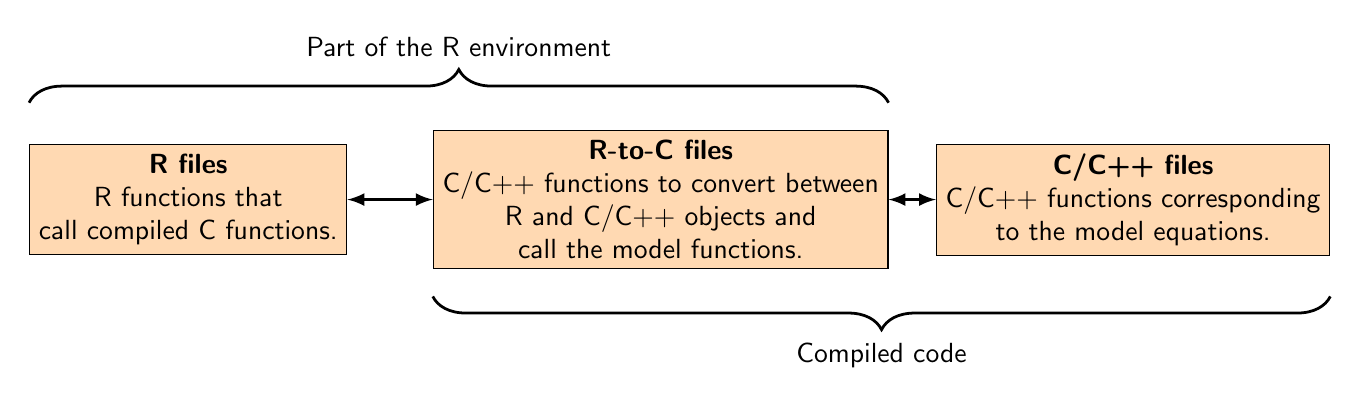
\begin{tikzpicture}[node distance=2 cm, decoration={brace}]
\tikzstyle{process} = [rectangle, minimum width=3 cm, minimum height=1 cm, text centered, draw=black, fill=orange!30]
\node (R)  [process, align=center] {\textbf{R files}\\R functions that\\call compiled C functions.};
\node (RC) [process, align=center, right of=R, xshift=4 cm] {\textbf{R-to-C files}\\C/C++ functions to convert between\\R and C/C++ objects and\\call the model functions.};
\node (C)  [process, align=center, right of=RC, xshift=4 cm] {\textbf{C/C++ files}\\C/C++ functions corresponding\\ to the model equations.};

\draw [latex-latex, line width=1.1 pt] (R) -- (RC);
\draw [latex-latex, line width=1.1 pt] (RC) -- (C);

\draw [decoration={brace, raise=10 pt, amplitude=12 pt}, decorate, line width=1 pt] (R.north west |- RC.north) -- node[above=23 pt] {Part of the R environment} (RC.east |- RC.north);
\draw [decoration={brace, raise=10 pt, amplitude=12 pt, mirror}, decorate, line width=1 pt] (RC.south west |- RC.south) -- node[below=23 pt] {Compiled code} (C.east |- RC.south);

\end{tikzpicture}
\end{center}
\end{figure}

R code should be written so that it only checks validity of arguments
and calls R-to-C functions. R-to-C code should only provide error
checking and call C/C++ functions. That is, R and R-to-C functions
should only provide a way to access the models written in C/C++, and
no modeling should be done in R or R-to-C code.

\subsection[Adding new models]{Adding new models\footnote{Up until
  now, we have (mostly) used the term \emph{model} to refer to the
  system as a whole, and the dynamics of how it changes over time.
  Here we are using it in a more specialized sense: we \emph{model}
  the relationship between attributes of a state---how the values of
  some select group of attributes of the state determine the values or
  the rate of change of the values of other attributes of the state.
  A model of the dynamics of soil evaporation, for instance, is a
  component of the model of the system as a whole.  When we are being
  careful, we will use the term \emph{module} to refer to the code (or
  the C++ class) that implements a \emph{model} (in this more
  restricted sense), but at times, we may use the two terms
  interchangably.}}

What follows are step-by-step instructions for writing modules and
integrating them into the BioCro library.  We show instructions both
for writing steady-state modules and for writing derivative modules.
In each case, we include a running example; the actual code changes
needed are shown in shadowboxes at the end of each step.  (Full
listings of the finished code are given in the appendix.)

Following this, we show instructions for writing tests of the new
modules.

\subsubsection{Example: Steps for creating a steady-state module.}

Suppose we want to write a module which builds upon the
\code{solar_zenith_angle} module.  That module, when given the
latitude, day of the year, and hour of the day as inputs, computes the
cosine of the solar zenith angle.  We would like to use the cosine of
the solar zenith angle to calculate the actual zenith angle in
degrees.  So we shall write a module taking one input,
``cosine\_zenith\_angle'', and computes the value of the angle itself.
The steps are as follows.

\begin{enumerate}

\item Decide on a name for the module.  While in theory, the name
  could be anything (ideally, something giving a concise description
  of the module), since we would like to follow the convention that
  the module name doubles as the name of the class that implements the
  module, the name (without quotes) should be a valid C++ identifier.%
  \footnote{
    The quoted name is the ``public'' name: when you specify
    the module in a BioCro R function, or if you use the BioCro C++
    library in your own C++ code, it is the string name---the quoted
    name---that you use.

    A valid C++ identifier must consist only of letters, digits and
    underscores; it cannot begin with a digit or match one of the C++
    keywords.  Additionally, to avoid conflicting with names reserved
    by the implementation, it should not begin with an underscore, and
    it should not contain a sequence of two or more underscores or an
    underscore followed by a capital letter; in fact, for the sake of
    uniformity, it is preferable to avoid capital letters in module
    names altogether.  Although non-latin letters are allowed, it is
    best to avoid them so encoding of source files does not become an
    issue.}

  \begin{example}[4]
    "solar_zenith_angle_in_degrees"
  \end{example}

\item Make a new file called \placeholder{module name}\code{.h} in the
  \code{src/module_library} directory.%
  \footnote{Here, and in what follows, we use italicized descriptors
    in angle brackets as placeholders for actual names or parts of
    names of files or variables.  So, for example, if we have chosen
    ``solar\_zenith\_angle\_in\_degrees'' as the module name, then
    \placeholder{module name}\code{.h} designates
    \code{solar_zenith_angle_in_degrees.h}.  Again, using the module
    name to form the file name is by convention, but a useful one if
    one is trying to find the code that implements a model.}

  \begin{example}[4]
    solar_zenith_angle_in_degrees.h
  \end{example}

\item Add appropriate header guards to the file.
  \begin{example}[4]
    #ifndef SOLAR_ZENITH_ANGLE_IN_DEGREES_H
    #define SOLAR_ZENITH_ANGLE_IN_DEGREES_H
    ...
    #endif
  \end{example}

\item Add \emph{include} directives to include the module base class
  declarations from \code{modules.h} and the type aliases from
  \code{state_map.h}.
  \begin{example}[4]
    #include "../modules.h"
    #include "../state_map.h"
  \end{example}

\item Begin a declaration of a class for the module, deriving it from
  SteadyModule.  The identifier used for the class name should match
  the module name you decided upon in step 1.\footnote{Here again,
  matching the class name to the module name is a convention.  It
  won't break anything if you don't except perhaps the expectations of
  readers of your code.}

  Include a Doxygen-style comment (that is, starting with \code{/**})
  describing the module and its purpose immediately above the class
  declaration.  The first sentence should be a brief summary of the
  module.  This is followed by additional details or a fuller
  description.  This is an appropriate place to include citations to
  sources for equations used by the module in calculations, the
  reasoning and justification for the model, and information to help
  the user determine when use of the model is
  appropriate.\footnote{The function that actually \emph{uses} the
  said equations will most likely be the \code{do_operation} function
  (or in some subsidiary function called by it).  But
  \code{do_operation} is a private function, so it is more appropriate
  to put ``public'' information here.  Documentation of
  \code{do_operation}, if any, should mostly be about programming
  details.}

  See section \ref{sec:doxygen} for how to quickly generate and view
  the documentation Doxygen produces from the documentation markup
  that you write.

  \begin{example}[4]
    /**
     *  Given a value for the BioCro variable "cosine_zenith_angle",
     *  compute and output a value for the variable
     *  "zenith_angle_in_degrees" that corresponds to the angle having
     *  the given cosine.
     *
     *  The module allows negative cosine values, corresponding to
     *  positions of the sun below the horizon.  If out-of-range values
     *  for the cosine are given, the output variable is set to NaN
     *  ("not-a-number").
     */
    class solar_zenith_angle_in_degrees : public SteadyModule {
      ...
      ...
      ...
    }
  \end{example}

\item Inside the body of the class declaration, declare private data
  members corresponding to the input and output parameters: Each
  member corresponding to an input parameter should be a reference of
  type \code{const double&}.\footnote{Most existing modules use
  pointers rather than references for the input parameter values.  But
  there is no reason not to use a reference, and it saves one from
  having to dereference the pointer when the value is used.}  By
  convention, the identifier used for the reference should be called
  \placeholder{parameter name}, that is, it should match the name of
  the corresponding parameter.%
  \footnote{There has been some discussion of relaxing this
    convention: As with module names, the (quoted) parameter name is
    the ``public-facing'' name known to users of the BioCro R
    functions or the BioCro C++ library.  As such, it might be
    desirable to be able to use more natural-sounding and descriptive
    names (and be able to include spaces!) rather than being confined
    to only using names the can be used in a C++ identifier.  In other
    words, it would be nice if these parameter names were
    ``user-centric'' instead of ``programmer-centric'': it is more
    user-centric, for example, to output simulation results with a
    column names like ``Relative Humidity'' and ``Temperature'' rather
    than ``rh'' and ``temp''.  (Your users will know without thinking
    that you aren't talking about blood types and temporary workers!)
    There may, however, be other better ways of addressing this
    issue.}
  Members corresponding to output parameters should be of type
  \code{double*} and should have names of the form
  \placeholder{parameter name}\code{_op}.\footnote{Be sure to consult
  the master parameter list to ensure you are using the input and
  output parameters correctly---that you are not assigning new
  meanings to existing parameters, and that the units you are
  expecting as input and that you wish to see in output match the
  units designated in that list.  \emph{If you are using a parameter
  whose name is not in that list, you will have to add it.}  [The
  afore-mentioned \emph{master parameter list} is, unfortunately, as
  of this writing, only slightly less fictional than Borges'
  \emph{Library of Babel}.]}

  \begin{example}[4]
    private:
       // References to input parameters:
       const double& cosine_zenith_angle;

       // Pointers to output parameters:
       double* zenith_angle_in_degrees_op;
  \end{example}

\item Declare a public constructor with signature
  \begin{C++listing}[4]
    |\placeholder{class name}|(const state_map* input_parameters, state_map* output_parameters)
  \end{C++listing}
  The constructor needs to initialize the base class
  \code{SteadyModule} with the name for the module, and each parameter
  variable needs to be initialized with an initializer of the form
  \begin{C++listing}[4]
    |\placeholder{parameter name}|{get_input(input_parameters, |\stringplaceholder{parameter name}|)}
  \end{C++listing}
  (for input parameters), or
  \begin{C++listing}[4]
    |\placeholder{parameter name}|_op{get_op(output_parameters, |\stringplaceholder{parameter name}|)}
  \end{C++listing}
  (for output parameters).%
  % This footnote was a real pain to typeset:
  \footnote{In existing modules, where pointers rather than references
      are used for input parameters, the initialization code will use
      the \code{get_ip} function instead of the \code{get_input}
      function:
      \placeholder{parameter name}\code{_ip}\{%
      \lstinline!get_ip(input_parameters,%
      !\ \stringplaceholder{parameter name})\}
  }

  \begin{example}[4]
    public:
       solar_zenith_angle_in_degrees(
           const state_map* input_parameters,
           state_map* output_parameters
       )
           : SteadyModule{"solar_zenith_angle_in_degrees"},
           cosine_zenith_angle{get_input(input_parameters, "cosine_zenith_angle")},
           zenith_angle_in_degrees_op{get_op(output_parameters, "zenith_angle_in_degrees")}
           {}
  \end{example}

\item Add the following static function declarations to the public
  section of the class body.
  \begin{example}[4]
    static string_vector get_inputs();
    static string_vector get_outputs();
  \end{example}

\item Add the following declaration to the private section to override
  the corresponding virtual function in the base class.
  \begin{example}[4]
    // Implement the pure virtual function do_operation():
    void do_operation() const override final;
  \end{example}

\item Implement \code{get_inputs()}; the function should return a
  vector of the names of all of the input parameters.  The function
  body can be just a return statement with the returned value written
  in the form of a \{\}-list, that is, a list of quoted strings of
  input parameter names, separated by commas and surrounded by curly
  braces.

  \begin{example}[4]
    string_vector solar_zenith_angle_in_degrees::get_inputs() {
        return {
            "cosine_zenith_angle"
        };
    }
  \end{example}

\item Implement \code{get_outputs()} similarly, returning a list of
  the names of all output parameters.
  \begin{example}[4]
    string_vector solar_zenith_angle_in_degrees::get_outputs() {
        return {
            "zenith_angle_in_degrees"
        };
    }
  \end{example}

\item Implement the \code{do_operation()} function.  This is the heart
  of the module---it's where the real work gets done.  Generally, the
  body of this function should contain a statement of the form
  \begin{C++listing}[4]
    update(|\placeholder{output parameter}|_op,|\placeholder{some value}|);
  \end{C++listing}
  for each output parameter.  Here, \placeholder{some value} is some
  numerical value calculated in the body of the function prior to the
  update statement, and it will generally be calculated from the
  values of the input parameters.  Computations often may entail the
  use of additional include directives, for example \code{\#include
  <cmath>} or \code{\#include "../constants.h"}.  In our example, the
  function definition (along with the required extra include
  directives) looks like this:
  \begin{example}[4]
    ...
    ...
    #include <cmath> // for acos
    #include "../constants.h" // for pi
    ...
    ...
    void solar_zenith_angle_in_degrees::do_operation() const {
        double zenith_angle { acos(cosine_zenith_angle)
                                * 180 / math_constants::pi };
        update(zenith_angle_in_degrees_op, zenith_angle);
    }
  \end{example}

\end{enumerate}

A listing of the completed module code is shown in appendix \ref{sza
  module listing}.

Once the new module has been written, it must be integrated into the
rest of the BioCro code.  This involves modifying the file
\code{module_library/module_wrapper_factory.cpp} and requires two
steps:

\begin{enumerate}

\item Add an include directive to include the header file for the new module.
  \begin{example}[4]
    #include "solar_zenith_angle_in_degrees.h"
  \end{example}

\item Add an entry to
  \code{module_wrapper_factory::module_wrapper_creators}.  This
  will be a bracketed pair of the form
  \begin{C++listing}[4]
    {|\stringplaceholder{module name}|, &create_wrapper<|\placeholder{module name}|>}
  \end{C++listing}

  \begin{example}[4]
    {"solar_zenith_angle_in_degrees", &create_wrapper<solar_zenith_angle_in_degrees>}
  \end{example}

\end{enumerate}

\subsubsection{Example: Steps for creating a derivative module.}

Suppose that we have weather data giving the ambient temperature over
some period of time and we wish to write a module to help us calculate
the (cumulative) number of heating degree days over that same period.
This is essentially the integral of the amount the ambient temperature
falls short of some ``threshold'' or ``base'' temperature, but
counting negative amounts as zero.  For this example, we will assume
that the ambient temperature is given in a variable called ``temp''
and the base temperature variable is named ``base\_temperature''.
These will be varying and unvarying known variables, respectively.

The steps for writing such a module are similar to those for writing a
steady-state module, but with some significant differences.

\begin{enumerate}

\item Decide on a name for the module.

  \begin{example}[4]
    "heating_degree_days"
  \end{example}

\item Make a new file called \placeholder{module name}.h in the
  \code{src/module_library} directory.

  \begin{example}[4]
    heating_degree_days.h
  \end{example}

\item Add appropriate header guards to the file.
  \begin{example}[4]
    #ifndef HEATING_DEGREE_DAYS_H
    #define HEATING_DEGREE_DAYS_H
    ...
    ...
    ...
    #endif
  \end{example}

\item Add include directives to include the module base class
  declarations from \code{modules.h} and the type aliases from
  \code{state_map.h}.
  \begin{example}[4]
    #include "../modules.h"
    #include "../state_map.h"
  \end{example}

\item Begin a declaration of a class for the module, deriving it from
  DerivModule.  The identifier used for the class name should match
  the module name you decided upon in step 1.
  \begin{example}[4]
    class heating_degree_days : public DerivModule {
      ...
      ...
      ...
    }
  \end{example}

\item Declare private data members corresponding to the input and
  output parameters.  Just as with steady-state modules, input
  parameter references should be of type \code{const double&} and by
  convention should have identifiers matching the parameter name.
  Output parameter pointers should be of type \code{double*} and
  should have names of the form \placeholder{parameter
  name}\code{_op}.
  \begin{example}[4]
    private:
       // References to input parameters:
       const double& temp;
       const double& base_temperature;

       // Pointers to output parameters:
       double* heating_degree_days_op;
  \end{example}

\item Declare a public constructor with signature
  \begin{C++listing}[4]
    |\placeholder{class name}|(const state_map* input_parameters, state_map* output_parameters)
  \end{C++listing}
  The constructor needs to initialize the base class
  \code{DerivModule} with the name for the module, and each parameter
  variable needs to be initialized with an initializer of the form
  \begin{C++listing}[4]
    |\placeholder{parameter name}|{get_input(input_parameters, |\stringplaceholder{parameter name}|)}
  \end{C++listing}
  (for input parameters), or
  \begin{C++listing}[4]
    |\placeholder{parameter name}|_op{get_op(output_parameters, |\stringplaceholder{parameter name}|)}
  \end{C++listing}
  (for output parameters).

  \begin{example}[4]
    public:
       heating_degree_days(
           const state_map*
               input_parameters,
           state_map*
               output_parameters
       )
       : DerivModule{"heating_degree_days"},
         temp{get_input(input_parameters, "temp")},
         base_temperature{get_input(input_parameters, "base_temperature")},
         heating_degree_days_op{get_op(output_parameters, "heating_degree_days")}
       {}
  \end{example}

\item Add the following static function declarations to the public
  section of the class body.
  \begin{example}[4]
    static string_vector get_inputs();
    static string_vector get_outputs();
  \end{example}

\item Add the following declaration to the private section to override
  the corresponding virtual function in the base class.
  \begin{example}[4]
    // Implement the pure virtual function do_operation():
    void do_operation() const override final;
  \end{example}

\item Implement \code{get_inputs()}; the function should return a
  vector of the names of all of the input parameters.  The function
  body can be just a return statement with the returned value written
  in the form of a \{\}-list, that is, a list of quoted strings of
  input parameter names, separated by commas and surrounded by curly
  braces.

  \begin{example}[4]
    string_vector heating_degree_days::get_inputs() {
        return {
            "temp",
            "base_temperature"
        };
    }
  \end{example}

\item Implement \code{get_outputs()} similarly, returning a list of
  the names of all output parameters.
  \begin{example}[4]
    string_vector heating_degree_days::get_outputs() {
        return {
            "heating_degree_days"
        };
    }
  \end{example}

\item Implement the \code{do_operation()} function.  This is the heart
  of the module---it's where the real work gets done.  Generally, the
  body of this function should contain a statement of the form
  \begin{C++listing}[4]
    update(|\placeholder{output parameter}|_op,|\placeholder{some value}|);
  \end{C++listing}
  for each output parameter.  Here, \placeholder{some value} is some
  numerical value calculated in the body of the function prior to the
  update statement, and it will generally be calculated from the
  values of the input parameters.  Since this is a \emph{derivative}
  module, it represents the \emph{rate of change \textbf{per hour}} of
  the output parameter.

  Computations
  often may entail the use of additional include directives, for
  example \code{\#include <cmath>} or \code{\#include
    "../constants.h"}.

  In our example, the function definition looks like this:
  \begin{example}[4]
    void heating_degree_days::do_operation() const {
        double temperature_deficit { base_temperature > temp ?
                                     (base_temperature - temp) : 0};

        update(heating_degree_days_op, temperature_deficit / 24.0);|\footnote{We must divide by 24 here because we want the rate of change of heating degree days \emph{per hour}.}%
        % Unfortunately, to get the footnote to work properly in this
        % context, it seems we must put it all on the same line.  (We
        % could use a \footnotemark / \footnotetext pair except
        % reverse links for footnotes doesn't currently seem to work
        % if one does that.
      |
    }
  \end{example}

\end{enumerate}

A listing of the completed module code is shown in appendix \ref{hdd
  module listing}.

The steps for integrating the module into the rest of the BioCro code
are exactly the same as for steady state modules, again only requiring
a few modifications to
\code{module_library/module_wrapper_factory.cpp}:

\begin{enumerate}

\item Add an include directive to include the header file for the new module.
  \begin{example}[4]
    #include "heating_degree_days.h"
  \end{example}

\item Add an entry to
  \code{module_wrapper_factory::module_wrapper_creators}.  This
  will be a bracketed pair of the form
  \begin{C++listing}[4]
    {|\stringplaceholder{module name}|, &create_wrapper<|\placeholder{module name}|>}
  \end{C++listing}
  \begin{example}[4]
    {"heating_degree_days", &create_wrapper<heating_degree_days>}
  \end{example}

\end{enumerate}

\subsubsection{Generating the Doxygen documentation}
\label{sec:doxygen}

If you go to the BioCro \code{documentation} directory and type
\code{make help} at the command line, you see information about
multiple options for generating and displaying the Doxygen
documentation in various configurations.  When you are in the process
of \emph{writing} documentation, however, it is convenient to be able
to quickly genererate the HTML- or PDF-style documents for just the
portion of the documentation you are working on.  One way to do this
is as follows.

Suppose we are working on the documentation in the module file
\begin{sh_listing}[2]
  src/module_library/solar_zenith_angle_in_degrees.h
\end{sh_listing}
Then we can quickly generate the HTML documentation for that file and
view it by issuing the command
\begin{sh_listing}[2]
  make source=../src/module_library/solar_zenith_angle_in_degrees.h \
       output_directory=minimal view
\end{sh_listing}

What we have done here is we have re-purposed the \code{make view}
command, which normally generates \emph{all} of the HTML documentation
for the C++ source code, and overridden the default set of documented
source files and the default documentation output directory so that we
only spend time generating the documentation for the file of interest
and so that the documentation is output to a different place (so that
it won't corrupt any existing documentation).  Thus, we set
\code{source} to the relative path to the file we are working on, and
we set \code{output} to the relative path to the directory under which
we want the documentation files to appear.\footnote{The name
\emph{minimal} for the output directory is arbitrary except that it is
best to choose a name that doesn't name an existing directory.
Overriding \emph{output} isn't strictly necessary, but if we don't,
the output will be written to
\code{documentation/doxygen_docs_complete}, a somewhat misleading name
for the minimal documentation we are generating.  Moreover, any
existing documentation in that location would be corrupted by the new
minimal documentation we generate.}

If we want to generate and view the PDF documentation, we could use
this command instead:
\begin{sh_listing}[2]
  make source=../src/module_library/solar_zenith_angle_in_degrees.h \
       output_directory=minimal view-pdf
\end{sh_listing}

\subsection{Writing tests for new models}
\label{sec:writing_tests}

Once a new module has been written, a set of unit tests should be
written to ensure that it works as expected.  For more about unit
tests in R, see \url{https://r-pkgs.org/tests.html}.  For general,
non-language-specific discussions of unit testing, see
\url{https://martinfowler.com/bliki/UnitTest.html} or
\url{https://builtin.com/software-engineering-perspectives/what-is-unit-testing}.


Here are step-by-step instructions for writing unit tests of modules,
using as examples the modules we have just written.\footnote{These
instructions are for testing in R.  It would be much more direct to
use a C++ testing framework to test C++ code; presumably such tests
could test the module functions independently of the rest of the
BioCro code, with a minimum of set-up and tear-down code.  But writing
tests in R is simpler.  Note, though, that this way of testing modules
depends on the correct functioning of the R interface to the BioCro
C++ library.  If the R front end is buggy, then the module tests may
fail for reasons not having anything to do with the underlying C++
module.}

\subsubsection{Writing unit tests for a steady-state module}
\label{sec:write_ss_unit_test}

  In writing our tests, we will make use of the R \Rcode{test_module}
  function.  This function takes as input the name of a module (as a
  string), and a list specifying values for all of the input
  parameters of the module.  It returns a list of values for the
  module's output parameters.

\begin{enumerate}

\item Create a file for the module tests in the directory
  \code{tests/testthat}.  The file name should begin with ``test-'' and
  end with ``.R''.  A good name for the file would be something of the
  form \code{test-}\placeholder{module name}\code{.R}.

  \begin{example}[4]
    test-solar_zenith_angle_in_degrees.R
  \end{example}

\item At the top of the new file, add a \emph{context} statement
  providing a general description of the tests in the file.  This
  will be a statement of the form
  \Rcode{context(}\stringplaceholder{some descriptive text}\Rcode{)}.

  \begin{Rexample}[4]
    context('Test basic functioning of the steady-state module "solar_zenith_angle_in_degrees".')
  \end{Rexample}

\item Write one or more tests.

  Each test will be a statement of the form
  \begin{Rlisting}[4]
    test_that(|\stringplaceholder{overall test description}|, {
      |\placeholder{one or more statements, including statements of the form \texttt{expect\_*(...)}}|
    })
  \end{Rlisting}

  More specifically, each test will generally set input parameter
  values for the module and then call
  \Rcode{test_module}:
  \begin{Rlisting}[4]
    result <- test_module(|\stringplaceholder{module name}|, |\placeholder{input parameter list}|)
  \end{Rlisting}
  The subsequent statements may then test various aspects of \Rcode{result}.

  The heart of a \Rcode{testthat} test are the \emph{expectations}.
  These are assertions of some condition that should hold or some
  result that should be obtained from running the module code.  They
  take the form of a function call to any one of a number of functions
  whose names begin with the string \Rcode{expect_}.  We will be
  primarily concerned with two such functions:
  \Rcode{expect_equal(}\placeholder{actual value}\Rcode{,}
  \placeholder{expected value}\Rcode{)}, which tests that its two
  arguments are equal (give or take some small amount, which can be
  specfied explicitely by supplying a third argument of the form
  \Rcode{tolerance =} \placeholder{some small number}); and
  \Rcode{expect_true(}\placeholder{some boolean condition}\Rcode{)},
  which tests that some condition holds.  More about \Rcode{expect_}
  functions can be found in the
  \href{https://r-pkgs.org/tests.html#expectations}{section on expect
  functions} in the book \href{https://r-pkgs.org/}{R Packages} by
  Hadley Wickham and Jenny Bryan; the full complement of
  \Rcode{expect_} functions is listed and documented at
  \url{https://cran.r-project.org/web/packages/testthat/testthat.pdf}.

  What should be tested?  Here are some possibilities:

  \begin{enumerate}

  \item Sample values that produce recognizable results.

    From elementary trignometry, we know, for example, that the angle
    between $0^\circ$ and $180^\circ$ having a cosine of $0.5$ is
    $60^\circ$.  We can test that this is the actual result obtained
    from our module with a simple test.  We can write our test as
    follows:

    \begin{Rexample}[6]
      test_that("When the cosine is 1/2, the angle is 60 degrees.", {
        input_parameters <- list(cosine_zenith_angle = 0.5)
        result = test_module("solar_zenith_angle_in_degrees", input_parameters)
        expect_equal(result$zenith_angle_in_degrees, 60)
      })
    \end{Rexample}

    Since we will likely call \Rcode{test_module} in each test, and
    with the same value for the module name each time, we can write a
    helper function to factor the repetitious code out of our tests;
    for example,

    \begin{Rexample}[6]
      angle_from_cosine <- function(cza) {
        input_parameters <- list(cosine_zenith_angle = cza)
        result <- test_module("solar_zenith_angle_in_degrees", input_parameters)
        result$zenith_angle_in_degrees
      }
    \end{Rexample}

    Then our test becomes simply

    \begin{Rexample}[6]
      test_that("When the cosine is 1/2, the angle is 60 degrees.", {
        angle <- angle_from_cosine(0.5)
        expect_equal(angle, 60)
      })
    \end{Rexample}


  \item Edge cases.

    It often makes sense to test module operation at the very
    limit of allowable values.  For the cosine of an angle, these
    limits are plus and minus one.\footnote{Note that zenith
      angles greater than $90^\circ$ correspond to the sun being
      below the horizon.}

    \begin{Rexample}[6]
      test_that("When the cosine is 1, the angle is 0 degrees", {
        angle <- angle_from_cosine(1)
        expect_equal(angle, 0)
      })

      test_that("When the cosine is -1, the angle is 180 degrees", {
        angle <- angle_from_cosine(-1)
        expect_equal(angle, 180)
      })
    \end{Rexample}

  \item It's a good idea to test how the module behaves when given
    input that is out of bounds.

    What should the module in our example do when given a value for
    the cosine that is greater than one or less than minus one?
    We'll assume it should return NaN (``not-a-number'').

    \begin{Rexample}[6]
      test_that("When the cosine is more than 1, the angle is not a number", {
        angle <- angle_from_cosine(1.000000001)
        expect_true(is.nan(angle))
      })

      test_that("When the cosine is less than -1, the angle is not a number", {
        angle <- angle_from_cosine(-1.000000001)
        expect_true(is.nan(angle))
      })
    \end{Rexample}

  \item Lastly, if you discover a bug in your module, it's a good
    idea to write a test that demonstrates the bug---a test that
    will pass once the bug is fixed and ensures it stays fixed if
    later changes are made.

  \end{enumerate}

  A listing of the complete test file is shown in appendix \ref{sza
    test file}.

\end{enumerate}


\subsubsection{Writing unit tests for a derivative module}
\label{sec:write_deriv_unit_test}

  Again, in writing our tests, we will make use of the R
  \Rcode{test_module} function. Keep in mind that in the case of a
  derivative module, the output values represent the rate of change of
  the output parameters \emph{per hour}. Here, we show how to test the
  heating degree days module.

\begin{enumerate}

\item Make a file for the test.

  \begin{Rexample}[4]
    test-heating_degree_days.R
  \end{Rexample}

\item Add a context statement.

  \begin{Rexample}[4]
    context('Test basic functioning of the derivative module "heating_degree_days".')
  \end{Rexample}

\item Write tests.

  A sample test file, with comments, for the
  \Rcode{heating_degree_days} module is shown in appendix \ref{hdd
    test file}.

\end{enumerate}

\subsubsection{Running the tests}

Perhaps the easiest way to run all of the \emph{testthat} tests is to
use the \emph{devtools} package: assuming you have an R session open
in a directory inside the BioCro source tree and \emph{devtools} has
been loaded, simply do this:

\begin{Rlisting}[2]
  test()
\end{Rlisting}

If you use RStudio, you needn't even type: choosing ``Test Package''
from the Build menu, or simply using the keyboard-shortcut ``Ctrl/Cmd
+ Shift + T'' will suffice.  This method of running the tests has the
added advantage that a test producing a segmentation fault won't crash
the whole R session.\footnote{If you don't have the devtools package
installed or haven't checked the "Use devtools package functions if
available" checkbox in the build configuration pane, the RStudio
``Test Package'' command will still work (assuming the \emph{testthat}
package itself has been installed), but it won't do quite the same
thing.  Instead of simply running all of the \Rcode{testthat} tests,
it will run all of the \Rcode{.R} files in the \Rcode{tests}
directory.  Since one of these files, \code{testthat.R}, runs all of
the \emph{testthat} tests, this will essentially amount to the same
thing unless there are other \Rcode{.R} files in the \code{tests}
directory.}

\Rcode{test()} will run all tests against the version of BioCro
represented by the source code.  To learn how to run the tests against
an \emph{installed} version, run the tests in only some of the files,
or avoid installing \emph{devtools}, consult the \emph{readme} file
\code{tests/README.md}.


\pagebreak



\begin{appendices}

\section{Writing unit tests using Gro\_solver}

The section on writing unit tests was originally written in such a way
that the tests called the \Rcode{Gro_solver} function.  This method of
testing a module entails setting up a complete system and running a
full simulation, albeit perhaps one with a very limited time span.

A much more convenient way to write tests is to use the
\Rcode{test_module} function. This is the method we demonstrate in
section~\ref{sec:writing_tests}.  By using \Rcode{test_module}, we can
test the basic functioning of a module while avoiding all of the many
steps needed to set up a full system for running a simulation.

There may be cases, however, where we may still want the flexibility
offered by being able to specify and run a full simulation.  Some of
the things we can do with a full-fledged system that we can't do just
by calling \Rcode{test_module} include

\begin{itemize}

\item testing how multiple modules work in conjunction with one
another

\item testing how the module chosen affects the evolution of a system
over time

\item testing how a module functions in the context of different
solvers

\end{itemize}

Thus, it may be useful to present the steps required to write a test
that sets up and runs a complete system; and so here, by way of some
simple examples, we re-present the material from section
\ref{sec:writing_tests}, this time showing how to write tests using
\Rcode{Gro_solver} instead of \Rcode{test_module}.  As an added
benefit, writing such tests will instruct a user in the rudiments of
setting up and running a simulation in BioCro.

\subsection{Writing a unit test for a steady-state module using
Gro\_solver}

For testing a steady-state module, it will suffice to set up a
bare-bones system: the sequence of states can be a sequence of length
one since we aren't interested in how the state changes over time.
And the state variables need only include the input variables for the
module being tested plus certain time-related variables.

\begin{itemize}

\item[1 \& 2.] Steps 1 and 2 are exactly as in section~\ref{sec:write_ss_unit_test}.

\end{itemize}

The third step is ``new'', as it involves setting up parameters for
the \Rcode{Gro_solver} function, something we don't need to do when
using \Rcode{test_module}:

\begin{enumerate}
\setcounter{enumi}{2}

\item Define parameters for the \Rcode{Gro_solver} function.  Assuming
  we call \Rcode{Gro_solver} as
  \begin{Rlisting}[4]
    Gro_solver(initial_state, invariant_parameters, varying_parameters,
               steady_state_modules, derivative_modules, solver, verbose)
  \end{Rlisting}
  we have seven variables we need to define:
  \begin{Rlisting}[4]
    initial_state <- ...
    invariant_parameters <- ...
    varying_parameters <- ...
    steady_state_modules <- ...
    derivative_modules <- ...
    solver <- ...
    verbose <- ...
  \end{Rlisting}

  (The last two have default values of
  \begin{Rlisting}[4]
    list(type='Gro', output_step_size=1.0, adaptive_rel_error_tol=1e-4, adaptive_abs_error_tol=1e-4, adaptive_max_steps=200)
  \end{Rlisting}
  and \Rcode{FALSE}, respectively.  Since it doesn't matter what
  solver we use for testing a steady state module, and since in
  general tests shouldn't produce their own output, these are suitable
  values and may be omitted.)\footnote{
    There may be cases where we may want to temporarily set
    \Rcode{verbose} to \Rcode{TRUE} in order to debug a test we are
    writing.  In this case, if we want to default the value of
    \Rcode{solver}, we must use a named argument to set the
    \Rcode{verbose} argument and write `\Rcode{verbose=TRUE}' instead
    of just `\Rcode{TRUE}' so that \Rcode{TRUE} is not taken to be the
    value for \Rcode{solver}.}

  What values should be used to fill in the blanks?  For the module
  lists, which are just vectors of names, the answer is clear:
  \begin{Rlisting}[4]
    steady_state_modules <- c(|\stringplaceholder{name of module being tested}|)
    derivative_modules <- c()
  \end{Rlisting}

  These may be defined globally, outside of any test.  The name of the
  module should exactly match the name as specified in the key of the
  entry for the module in \code{module_wrapper_creators}.

  In our example, we use

  \begin{Rexample}[4]
    steady_state_modules <- c("solar_zenith_angle_in_degrees")
    derivative_modules <- c()
  \end{Rexample}


  On the other hand, values for the module input parameters and for
  the initial state may potentially vary with each test.  The keys,
  however, will in most cases be uniform across tests.  For example,
  if the module inputs consist of invariant parameters $\ip_1$,
  $\ip_2$, \dots, $\ip_k$, varying parameters $\vp_1$, $\vp_2$, \dots,
  $\vp_m$, and initial state variables $\isv_1$, $\isv_2$, \dots,
  $\isv_n$, then we will be setting the corresponding function
  parameters to values of the following forms:
  \begin{Rlisting}[4]
    invariant_parameters <- list(ip_1 = ___, ip_2 = ___, ..., ip_k = ___)
    varying_parameters <- list(vp_1 = ___, vp_2 = ___, ..., vp_m = ___)
    initial_state <- list(isv_1 = ___, isv_2 = ___, ..., isv_n = ___)
  \end{Rlisting}

  As mentioned above, since we are setting up the most stripped-down
  of systems, these lists will be very short: we need to include a
  setting for each input parameter of the module being tested, and we
  need to include certain time-related settings.  In particular, the
  invariant parameter list must include a setting for
  \Rcode{timestep}, and the varying parameters must include either a
  setting for \Rcode{time} or for both \Rcode{doy} and
  \Rcode{hour}.  The values assigned to the time-related variables is
  immaterial for the purposes of the test except in the case that one
  of them is also an input to the module being tested.  (The
  \code{solar_zenith_angle} module, for example, takes \Rcode{time}
  as an input.)  It is best, however, to assign values that might make
  sense in the simulation of a ``real'' system.

  As for which list should include the module input variable values,
  this too is largely immaterial for the purposes of running the test.
  But again, to minimize confusion, it is best to include the setting
  in the list that would make sense in a real system.  So, for
  example, if it is a parameter that normally varies over the course
  of time, then it doesn't make sense to assign it in the
  \Rcode{invariant_parameters} list, and if it varies over time but
  not in a way that can be predicted from rates of change, then it
  shouldn't be assigned within the \Rcode{initial_state}.

  For our example, we use settings as follows.

  \begin{Rexample}[4]
    invariant_parameters <- list(timestep = 1)
    varying_parameters <- list(time = 1,
                               cosine_zenith_angle = |\placeholder{some value that will vary from test to test}|)
    initial_state <- list()
  \end{Rexample}

\item Write one or more tests.

  As in section~\ref{sec:write_ss_unit_test}, each test will be a
  statement of the form
    \begin{Rlisting}[4]
    test_that(|\stringplaceholder{overall test description}|, {
      |\placeholder{one or more statements, including statements of the form \texttt{expect\_*(...)}}|
    })
  \end{Rlisting}
  However, instead of getting results to test by calling
  \Rcode{test_module}, we call \Rcode{Gro_solver} instead:
  \begin{Rlisting}[4]
    result = Gro_solver(initial_state, invariant_parameters, varying_parameters, steady_state_modules, derivative_modules)
  \end{Rlisting}

As before, the various \Rcode{expect_} functions are used to test
\Rcode{result}.  In fact, once we make some global parameter settings
and re-define our helper function \Rcode{angle_from_cosine} to utilize
\Rcode{Gro_solver} instead of \Rcode{test_module}, the tests
themselves can remain exactly as in section~\ref{sec:write_ss_unit_test}.

Here are the precise settings we will use for the modules, invariant
parameters, and initial state:

    \begin{Rexample}[6]
      steady_state_modules <- c("solar_zenith_angle_in_degrees")
      derivative_modules <- c()

      initial_state <- list()
      invariant_parameters <- list(timestep = 1)
    \end{Rexample}

The helper function \Rcode{angle_from_cosine} becomes:\footnote{
      We make no attempt here to coordinate the input
      values for \Rcode{cosine_zenith_angle} and for
      \Rcode{time}. While in general we prefer to use input
      values that might be associated with a realistic system, for
      the purposes of writing tests of a module, it may sometimes be
      more convenient not to do so.}

    \begin{Rexample}[6]
      angle_from_cosine <- function(cza) {
        varying_parameters <- list(time = 1, cosine_zenith_angle = cza)
        result = Gro_solver(initial_state, invariant_parameters, varying_parameters, steady_state_modules, derivative_modules)
        result$zenith_angle_in_degrees
      }
    \end{Rexample}

  A listing of the complete test file is shown in appendix~\ref{szags
    test file}.

\end{enumerate}


\subsection{Writing unit tests for a derivative module using Gro\_solver}

Again, it will suffice to set up a bare-bones system.  But this time,
we will set up a time sequence of length two or more since we want to
see how the derivative affects how the state changes over time.  For
the most basic tests of module functionality, we need only use a
sequence of two states.  Again, the state variables need only include
the input variables for the module being tested and the time-related
variables.\footnote{
  In the case of a derivative module where some of the inputs
  correspond to outputs of steady-state modules, we have two choices
  with regard to testing: (1) include, as part of the test,
  steady-state modules that produce these required inputs; (2)
  artificially include values for these inputs as part of the varying
  parameters.  The latter option is the simplest and has the advantage
  of narrowing the scope of the test to the module we are most
  interested in testing.  But there may be cases where we want to test
  how two or more modules work in conjunction with one another.}

Here, we show how to test the heating degree days module using \Rcode{Gro_solver}.

\begin{itemize}

\item[1 \& 2.] Steps 1 and 2 are exactly the same as in
        section~\ref{sec:write_deriv_unit_test}.

\end{itemize}

Again, we need an extra step for setting up some \Rcode{Gro_solver} parameters:

\begin{enumerate}
\setcounter{enumi}{2}

\item Define parameters for the \Rcode{Gro_solver} function.  Again,
  we will be assuming we call \Rcode{Gro_solver} with
  \begin{Rlisting}[4]
    Gro_solver(initial_state, invariant_parameters, varying_parameters,
               steady_state_modules, derivative_modules, solver, verbose)
  \end{Rlisting}

  The assignments for the two module vectors are more or less the
  reverse of what they were for the steady-state module test:
  \begin{Rlisting}[4]
    steady_state_modules <- c()
    derivative_modules <- c(|\stringplaceholder{name of module being tested}|)
  \end{Rlisting}

  For our example, this becomes
  \begin{Rexample}[4]
    steady_state_modules <- c()
    derivative_modules <- c("heating_degree_days")
  \end{Rexample}

  As for \Rcode{initial_state}, \Rcode{invariant_parameters}, and
  \Rcode{varying_parameters}, we may want to vary each of these from
  test to test.  We may also want to run tests using various solvers
  and vary the timestep.

  For our example, we'll write a global helper function that makes this easy.

  \begin{Rexample}[4]
    calculate_heating_degree_days <- function(initial_value, time_vector, temperature_vector, threshold_temperature, timestep, solver) {
      initial_state <- list(heating_degree_days = initial_value)
      invariant_parameters <- list(base_temperature = threshold_temperature, timestep = timestep)
      varying_parameters <- list(time = time_vector, temp = temperature_vector)

      result <- Gro_solver(initial_state, invariant_parameters, varying_parameters,
                           steady_state_modules, derivative_modules, solver)

      result$heating_degree_days[length(time_vector)]
    }
  \end{Rexample}

\item Write tests.

  A sample test file, with comments, for the
  \Rcode{heating_degree_days} module is shown in appendix \ref{hddgs
  test file}.

\end{enumerate}


\section{Code listings}

\subsection{Full listing of solar-zenith-angle-in-degrees module} \label{sza module listing}

(In this listing, we have expanded the class's Doxygen comment to
demonstrate how LaTeX-style equations could be included, if desired.
See section \ref{sec:doxygen} for instructions on how to quickly and
easily generate and display the resulting HTML and PDF forms of the
Doxygen documentation.)

\lstinputlisting[style=C++style]{an_introduction_to_biocro/solar_zenith_angle_in_degrees.h}

\subsection{Full listing of heating-degree-days module} \label{hdd module listing}

\lstinputlisting[style=C++style]{an_introduction_to_biocro/heating_degree_days.h}

\subsection{Full listing of the unit-test file for solar-zenith-angle-in-degrees} \label{sza test file}

\lstinputlisting[style=Rstyle]{an_introduction_to_biocro/test-solar_zenith_angle_in_degrees.R}

\subsection{Full listing of the unit-test file for heating-degree-days} \label{hdd test file}

\lstinputlisting[style=Rstyle]{an_introduction_to_biocro/test-heating_degree_days.R}

\subsection{Full listing of the unit-test file for solar-zenith-angle-in-degrees---Gro\_solver version} \label{szags test file}

\lstinputlisting[style=Rstyle]{an_introduction_to_biocro/test-solar_zenith_angle_in_degrees_with_Gro_solver.R}

\subsection{Full listing of the unit-test file for heating-degree-days---Gro\_solver version} \label{hddgs test file}

\lstinputlisting[style=Rstyle]{an_introduction_to_biocro/test-heating_degree_days_with_Gro_solver.R}

\end{appendices}

\end{document}
